% ==============================================================================
% MANSUETO SHORT DECK
% ==============================================================================

\begin{frame}
    \frametitle{Motivation}
    \begin{minipage}{0.48\textwidth}
        \begin{figure}
            \centering
            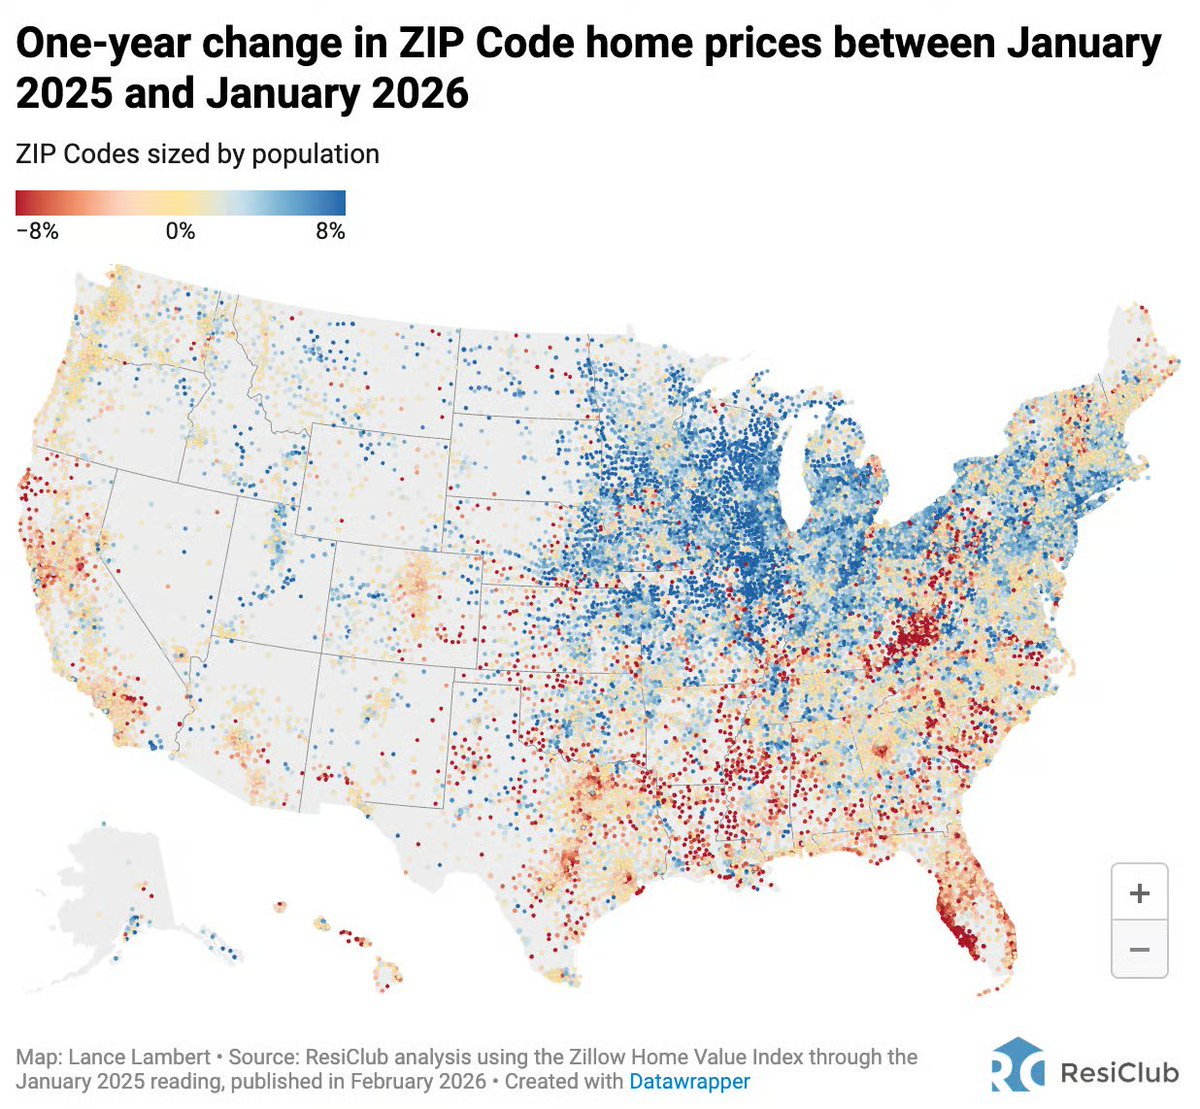
\includegraphics[width=\textwidth,height=0.8\textheight,keepaspectratio]{../slides/images/home_price_growth.png}
        \end{figure}
    \end{minipage}
    \hfill
    \begin{minipage}{0.48\textwidth}
        \begin{figure}
            \centering
            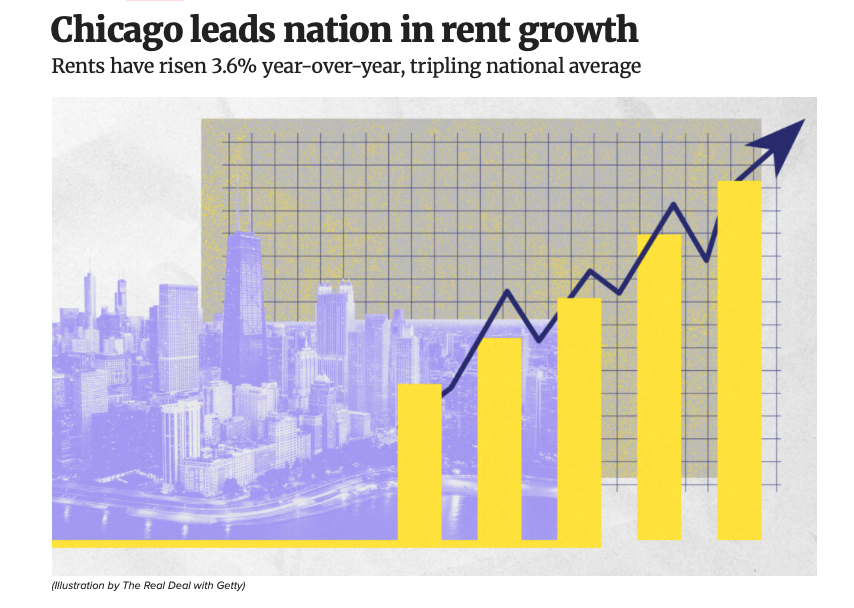
\includegraphics[width=\textwidth,height=0.8\textheight,keepaspectratio]{../slides/images/rent_growth_headline.png}
        \end{figure}
    \end{minipage}
\end{frame}

\begin{frame}
    \frametitle{Motivation}
    \begin{itemize}
        \item Housing prices and rents are rising sharply in many U.S.\ cities, including Chicago
        \begin{itemize}
            \item Limited housing supply in high-demand areas is widely viewed as a key driver
            \item Land-use regulation and local control are often blamed for limiting supply
        \end{itemize}
        \item Most research focuses on formal rules such as by-right zoning
        \begin{itemize}
            \item Discretionary regulation can also shape development, but is harder to measure
        \end{itemize}
        \item \textbf{Chicago}: aldermanic privilege creates sharp, local variation in de facto regulatory stringency
    \end{itemize}
\end{frame}

\begin{frame}
    \frametitle{What is Aldermanic Privilege?}
    \begin{columns}[T]
    \begin{column}{0.58\textwidth}
        \textbf{City council logistics}
        \begin{itemize}\setlength{\itemsep}{2pt}
            \item 50 wards + aldermen, each elected only by their ward's residents
            \item $\sim$50,000 people per ward; 4-year terms but often decades in office
        \end{itemize}
        \vspace{0.3em}
        \textbf{Key feature: Deference}
        \begin{itemize}\setlength{\itemsep}{2pt}
            \item ``Very few things happen that aldermen don't want to happen.'' \mbox{\scriptsize \citep{zhang_boundaries_2011}}
            \item Often referred to as ``little mayors'' ruling wards as ``fiefdoms''
            \item Chicago's aldermen have \textbf{more discretion} over local development than politicians in many peer U.S.\ cities
        \end{itemize}
    \end{column}
    \begin{column}{0.40\textwidth}
        \centering
        \includegraphics[width=\textwidth,height=0.82\textheight,keepaspectratio]{../tasks/audits/ward_map/output/ward_map_2024.pdf}
    \end{column}
    \end{columns}
\end{frame}

\begin{frame}
    \frametitle{Aldermanic Privilege is a Hotly Contested Issue in Chicago}
    \begin{minipage}{0.5\textwidth}
        \begin{figure}
            \centering
            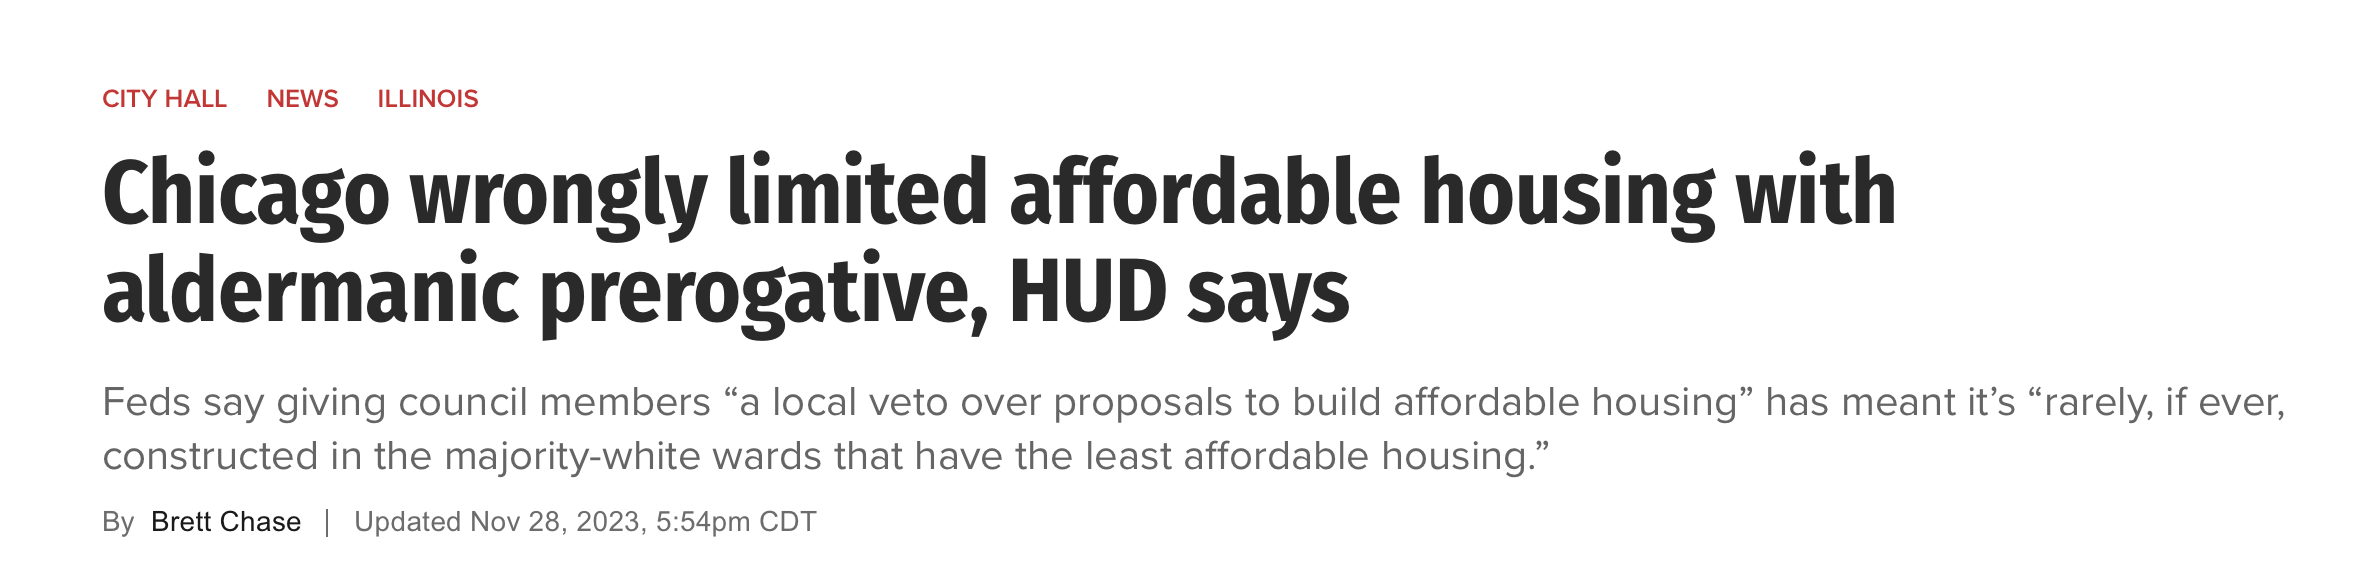
\includegraphics[width=\textwidth]{../slides/images/hud_report_headline.png}
        \end{figure}
        \begin{figure}
            \centering
            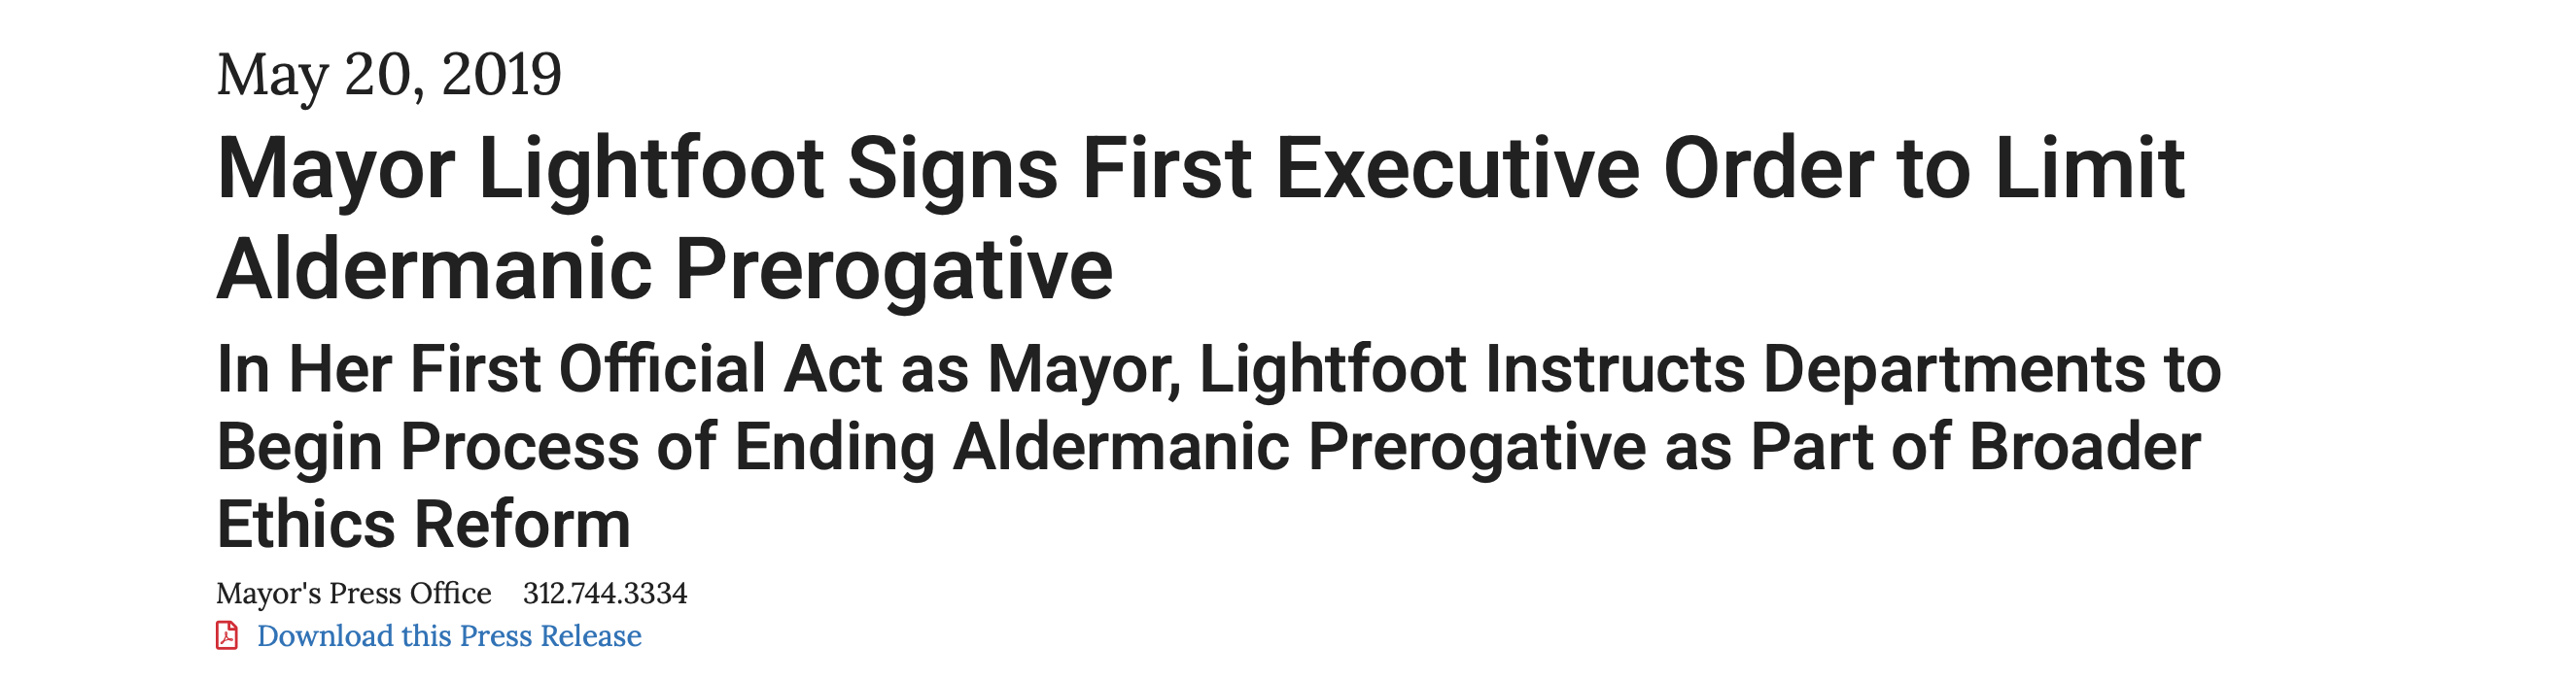
\includegraphics[width=\textwidth]{../slides/images/lightfoot_order.png}
        \end{figure}
        \begin{figure}
            \centering
            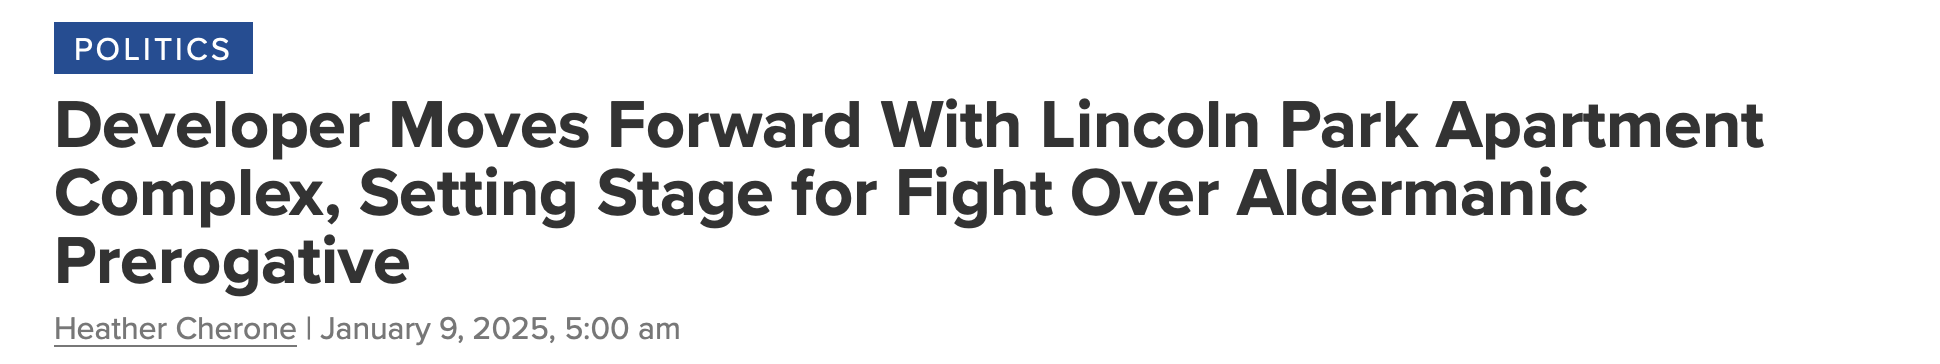
\includegraphics[width=\textwidth]{../slides/images/alderman_fight.png}
        \end{figure}
    \end{minipage}
    \hfill
    \begin{minipage}{0.48\textwidth}
        \begin{figure}
            \centering
            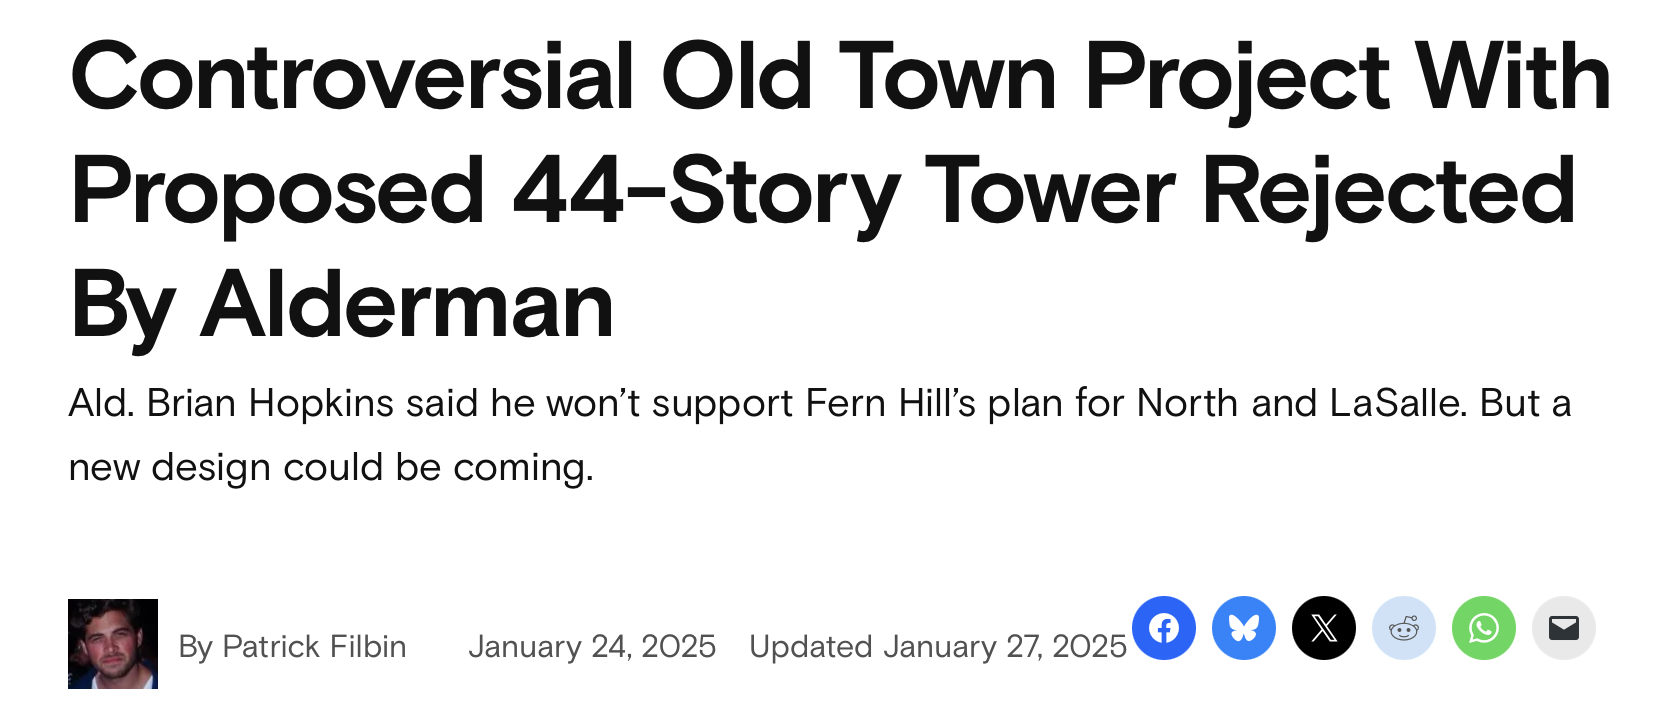
\includegraphics[width=\textwidth]{../slides/images/old_town_towers.png}
        \end{figure}
        \begin{figure}
            \centering
            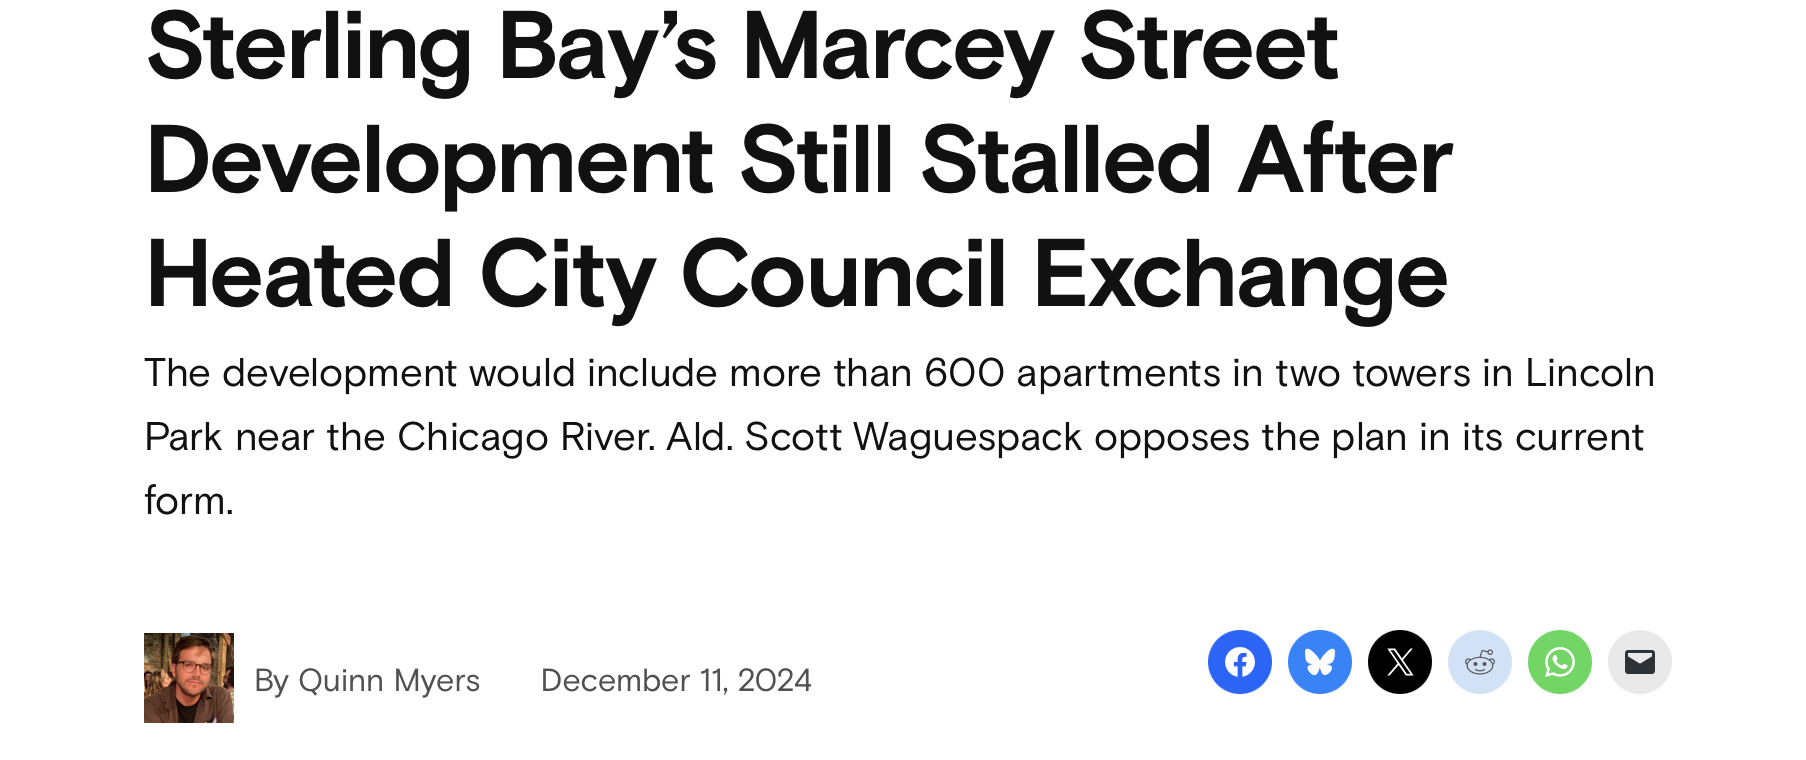
\includegraphics[width=\textwidth]{../slides/images/sterling_bay_fight.png}
        \end{figure}
    \end{minipage}
\end{frame}

\begin{frame}
    \frametitle{Roadmap}
    \textbf{What I do}
    \begin{itemize}[itemsep=.4em,topsep=0.8em]
        \item I use variation in alderman-level permit processing times to construct a measure of regulatory stringency across wards
        \item Use ward boundary discontinuities and redistricting events to estimate the effect of regulatory stringency on housing supply, rents, and home prices
    \end{itemize}

    \vspace{0.3em}

    \textbf{Preview of results}
    \begin{itemize}[itemsep=.4em,topsep=0.8em]
        \item I find that moving to the stringent side of a ward boundary reduces multifamily density by 12-14\% and permits by 7\%
        \item This appears to pass through into higher rents and home prices
    \end{itemize}
\end{frame}

\begin{frame}[label=permit-stats-main]
    \frametitle{Why Permit Processing Times?}
    \begin{columns}[T]
    \begin{column}{0.46\textwidth}
        \begin{itemize}[itemsep=0.2em,topsep=0.25em]
            \item Permitting is a primary driver of supply inelasticity \citep{soltas_how_2026}
            \item Focus on \textbf{high-discretion} permits: new construction, renovation, and demolition
        \end{itemize}
        \vspace{0.65em}
        {\scriptsize
        \centering
        \textbf{Mean processing time vs.\ ward-month permit volume}
        \vspace{0.15em}

        \setlength{\tabcolsep}{3pt}
        \renewcommand{\arraystretch}{1.05}
        \begin{tabular}{lr}
            \toprule
            Permit group & Corr. \\
            \midrule
            High-discretion & -0.123 \\
            Low-discretion & 0.106 \\
            All permits & -0.021 \\
            \bottomrule
        \end{tabular}
        \par}
    \end{column}
    \begin{column}{0.52\textwidth}
        \begin{itemize}[itemsep=0.45em,topsep=0.25em]
            \item I residualize log processing time on ward demographics, geography, lagged volume, plus month and permit characteristic FEs.
            \item I then take those residuals and regress them on alderman dummies to create alderman fixed effects, and use Empirical Bayes shrinkage to reduce noisy estimates.
        \end{itemize}
    \end{column}
    \end{columns}
\end{frame}

\begin{frame}
    \frametitle{Stringency Score Results}
    \begin{columns}[T]
    \begin{column}{0.48\textwidth}
        \centering
        
        \vspace{0.1em}

        \includegraphics[width=\textwidth,height=0.70\textheight,keepaspectratio]{../tasks/within_ward_strictness/output/predecessor_successor_scatter_uncertainty_ptfeTRUE_rtfeTRUE_porchTRUE_cafeFALSE_2stage_volLAG1_BOTH_through2022.pdf}
    \end{column}
    \begin{column}{0.49\textwidth}
        \centering
        
        \vspace{0.1em}

        \includegraphics[width=\textwidth,height=0.70\textheight,keepaspectratio,trim=0.12cm 0cm 0.12cm 0cm,clip]{../tasks/strictness_score_map/output/uncertainty_score_map_ptfeTRUE_rtfeTRUE_porchTRUE_cafeFALSE_2stage_volLAG1_BOTH_through2022_2022-01.pdf}
    \end{column}
    \end{columns}
\end{frame}

\begin{frame}[label=visual-rd-main]
    \frametitle{Density Falls at Ward Borders; Larger for Multifamily}
    \begin{center}
        \includegraphics[width=0.94\textwidth,height=0.72\textheight,keepaspectratio]{../tasks/nonparametric_rd_density_linear_display/output/nonparametric_rd_density_linear_display_4panel_500ft_all_multifamily_bins5.pdf}
    \end{center}
    \scriptsize
    \textit{Notes}: 500 ft bandwidth. Regression includes zoning-group, segment, and year fixed effects along with demographic controls. 
\end{frame}

\begin{frame}
    \frametitle{Redistricting Treatment}
    \begin{center}
        \textbf{Ward pair 13-23 treatment example}
        \vspace{0.2em}

        \includegraphics[width=0.72\textwidth,height=0.62\textheight,keepaspectratio]{../tasks/event_study_treatment_maps/output/ward_pair_vertical_13-23_1000ft.pdf}
    \end{center}
    \vspace{-0.2em}
    \scriptsize
    Blocks that switch aldermen are compared to nearby blocks that remain in the origin ward; treatment intensity is the change in alderman stringency.
\end{frame}

\begin{frame}
    \frametitle{Permit Event Study}
    \begin{center}
        \begin{tikzpicture}
            \node[anchor=south west,inner sep=0] (plot) at (0,0) {
                \includegraphics[width=0.72\textwidth,height=0.68\textheight,keepaspectratio]{../tasks/run_event_study_permit/output/event_study_yearly_cohort_2015_high_discretion_issue_ppml_continuous_uniform_1000ft_within_block_full_clust_block_geo_wardpair.pdf}
            };
            \node[anchor=north east,align=left,fill=white,draw=gray!35,inner sep=3pt,font=\scriptsize] at ($(plot.north east)+(-0.25,-0.45)$) {
                \begin{tabular}{@{}l@{}}
                    Pooled Est: $-0.0768^{**}$ \\
                    \hspace{45pt} $(0.0365)$
                \end{tabular}
            };
        \end{tikzpicture}
    \end{center}
    \vspace{-1.0em}
    \scriptsize
    \[
    \log E[Y_{bt}]
    = \alpha_b + \lambda_{g(b)t}
    + \sum_{\tau \neq -1}\beta_\tau
    \left(\Delta \text{Stringency}_b \times \mathbf{1}\{t = \tau\}\right)
    \]
\end{frame}

\begin{frame}
    \frametitle{Rents are Higher on the More Stringent Side}
    \begin{center}
        \includegraphics[width=0.92\textwidth,height=0.72\textheight,keepaspectratio]{../tasks/rental_rd/output/rental_rd_flat_bw500_2014_2022_all_controls.pdf}
    \end{center}
    \vspace{-0.3em}
    \scriptsize
     500 ft bandwidth. Regression includes segment-by-month fixed effects along with hedonic and demographic controls. 
\end{frame}

\begin{frame}
    \frametitle{Home Prices also Show a Small Discontinuity}
    \begin{center}
        \includegraphics[width=0.92\textwidth,height=0.72\textheight,keepaspectratio]{../tasks/sales_border_pair_fe/output/sales_rd_flat_bw500_year_quarter_amenity_clust_segment.pdf}
    \end{center}
    \vspace{-0.3em}
    \scriptsize
    500 ft bandwidth. Regression includes segment-by-quarter fixed effects along with hedonic and demographic controls. 
\end{frame}

\begin{frame}[shrink=8]
    \frametitle{Conclusion}

    \textbf{Summary of findings}:
    \begin{itemize}[itemsep=0.12em,topsep=0.15em]
        \item Substantial variation in regulatory discretion across wards in Chicago
        \item Leads to $12-14\%$ less multifamily density and $7\%$ fewer permits in wards with more stringent aldermen
        \item Suggestive evidence that these frictions lead to higher rents and home prices in the city
    \end{itemize}

    \vspace{0.15em}
    \textbf{Implications}:
    \begin{itemize}[itemsep=0.12em,topsep=0.15em]
        \item Regulatory discretion, which manifests in discrete changes in regulatory stringency across the city, lowers density + housing supply and raises rents
        \item Within-city variation in the regulatory environment matters, not just cross-municipality differences
        \item Reforms should target decision-making authority and discretion, not just by-right zoning reforms
    \end{itemize}

\end{frame}
